\documentclass[11pt,a4paper,]{article}
\usepackage{lmodern}

\usepackage{amssymb,amsmath}
\usepackage{ifxetex,ifluatex}
\usepackage{fixltx2e} % provides \textsubscript
\ifnum 0\ifxetex 1\fi\ifluatex 1\fi=0 % if pdftex
  \usepackage[T1]{fontenc}
  \usepackage[utf8]{inputenc}
\else % if luatex or xelatex
  \usepackage{unicode-math}
  \defaultfontfeatures{Ligatures=TeX,Scale=MatchLowercase}
\fi
% use upquote if available, for straight quotes in verbatim environments
\IfFileExists{upquote.sty}{\usepackage{upquote}}{}
% use microtype if available
\IfFileExists{microtype.sty}{%
\usepackage[]{microtype}
\UseMicrotypeSet[protrusion]{basicmath} % disable protrusion for tt fonts
}{}
\PassOptionsToPackage{hyphens}{url} % url is loaded by hyperref
\usepackage[unicode=true]{hyperref}
\hypersetup{
            pdftitle={Assignment 4 ggplot2},
            pdfborder={0 0 0},
            breaklinks=true}
\urlstyle{same}  % don't use monospace font for urls
\usepackage{geometry}
\geometry{a4paper, centering, text={16cm,24cm}}
\usepackage[style=authoryear-comp,]{biblatex}
\addbibresource{references.bib}
\usepackage{longtable,booktabs}
% Fix footnotes in tables (requires footnote package)
\IfFileExists{footnote.sty}{\usepackage{footnote}\makesavenoteenv{long table}}{}
\usepackage{graphicx,grffile}
\makeatletter
\def\maxwidth{\ifdim\Gin@nat@width>\linewidth\linewidth\else\Gin@nat@width\fi}
\def\maxheight{\ifdim\Gin@nat@height>\textheight\textheight\else\Gin@nat@height\fi}
\makeatother
% Scale images if necessary, so that they will not overflow the page
% margins by default, and it is still possible to overwrite the defaults
% using explicit options in \includegraphics[width, height, ...]{}
\setkeys{Gin}{width=\maxwidth,height=\maxheight,keepaspectratio}
\IfFileExists{parskip.sty}{%
\usepackage{parskip}
}{% else
\setlength{\parindent}{0pt}
\setlength{\parskip}{6pt plus 2pt minus 1pt}
}
\setlength{\emergencystretch}{3em}  % prevent overfull lines
\providecommand{\tightlist}{%
  \setlength{\itemsep}{0pt}\setlength{\parskip}{0pt}}
\setcounter{secnumdepth}{5}

% set default figure placement to htbp
\makeatletter
\def\fps@figure{htbp}
\makeatother


\title{Assignment 4 ggplot2}

%% MONASH STUFF

%% CAPTIONS
\RequirePackage{caption}
\DeclareCaptionStyle{italic}[justification=centering]
 {labelfont={bf},textfont={it},labelsep=colon}
\captionsetup[figure]{style=italic,format=hang,singlelinecheck=true}
\captionsetup[table]{style=italic,format=hang,singlelinecheck=true}


%% FONT
\RequirePackage{bera}
\RequirePackage[charter,expert,sfscaled]{mathdesign}
\RequirePackage{fontawesome}

%% HEADERS AND FOOTERS
\RequirePackage{fancyhdr}
\pagestyle{fancy}
\rfoot{\Large\sffamily\raisebox{-0.1cm}{\textbf{\thepage}}}
\makeatletter
\lhead{\textsf{\expandafter{\@title}}}
\makeatother
\rhead{}
\cfoot{}
\setlength{\headheight}{15pt}
\renewcommand{\headrulewidth}{0.4pt}
\renewcommand{\footrulewidth}{0.4pt}
\fancypagestyle{plain}{%
\fancyhf{} % clear all header and footer fields
\fancyfoot[C]{\sffamily\thepage} % except the center
\renewcommand{\headrulewidth}{0pt}
\renewcommand{\footrulewidth}{0pt}}

%% MATHS
\RequirePackage{bm,amsmath}
\allowdisplaybreaks

%% GRAPHICS
\RequirePackage{graphicx}
\setcounter{topnumber}{2}
\setcounter{bottomnumber}{2}
\setcounter{totalnumber}{4}
\renewcommand{\topfraction}{0.85}
\renewcommand{\bottomfraction}{0.85}
\renewcommand{\textfraction}{0.15}
\renewcommand{\floatpagefraction}{0.8}


%\RequirePackage[section]{placeins}

%% SECTION TITLES


%% SECTION TITLES (NEW: Changing sections and subsections color)
\RequirePackage[compact,sf,bf]{titlesec}
\titleformat*{\section}{\Large\sf\bfseries\color[rgb]{0.8, 0.7, 0.1 }}
\titleformat*{\subsection}{\large\sf\bfseries\color[rgb]{0.8, 0.7, 0.1 }}
\titleformat*{\subsubsection}{\sf\bfseries\color[rgb]{0.8, 0.7, 0.1 }}
\titlespacing{\section}{0pt}{2ex}{.5ex}
\titlespacing{\subsection}{0pt}{1.5ex}{0ex}
\titlespacing{\subsubsection}{0pt}{.5ex}{0ex}


%% TITLE PAGE
\def\Date{\number\day}
\def\Month{\ifcase\month\or
 January\or February\or March\or April\or May\or June\or
 July\or August\or September\or October\or November\or December\fi}
\def\Year{\number\year}

%% LINE AND PAGE BREAKING
\sloppy
\clubpenalty = 10000
\widowpenalty = 10000
\brokenpenalty = 10000
\RequirePackage{microtype}

%% PARAGRAPH BREAKS
\setlength{\parskip}{1.4ex}
\setlength{\parindent}{0em}

%% HYPERLINKS
\RequirePackage{xcolor} % Needed for links
\definecolor{darkblue}{rgb}{0,0,.6}
\RequirePackage{url}

\makeatletter
\@ifpackageloaded{hyperref}{}{\RequirePackage{hyperref}}
\makeatother
\hypersetup{
     citecolor=0 0 0,
     breaklinks=true,
     bookmarksopen=true,
     bookmarksnumbered=true,
     linkcolor=darkblue,
     urlcolor=blue,
     citecolor=darkblue,
     colorlinks=true}

\usepackage[showonlyrefs]{mathtools}
\usepackage[no-weekday]{eukdate}

%% BIBLIOGRAPHY

\makeatletter
\@ifpackageloaded{biblatex}{}{\usepackage[style=authoryear-comp, backend=biber, natbib=true]{biblatex}}
\makeatother
\ExecuteBibliographyOptions{bibencoding=utf8,minnames=1,maxnames=3, maxbibnames=99,dashed=false,terseinits=true,giveninits=true,uniquename=false,uniquelist=false,doi=false, isbn=false,url=true,sortcites=false}

\DeclareFieldFormat{url}{\texttt{\url{#1}}}
\DeclareFieldFormat[article]{pages}{#1}
\DeclareFieldFormat[inproceedings]{pages}{\lowercase{pp.}#1}
\DeclareFieldFormat[incollection]{pages}{\lowercase{pp.}#1}
\DeclareFieldFormat[article]{volume}{\mkbibbold{#1}}
\DeclareFieldFormat[article]{number}{\mkbibparens{#1}}
\DeclareFieldFormat[article]{title}{\MakeCapital{#1}}
\DeclareFieldFormat[article]{url}{}
%\DeclareFieldFormat[book]{url}{}
%\DeclareFieldFormat[inbook]{url}{}
%\DeclareFieldFormat[incollection]{url}{}
%\DeclareFieldFormat[inproceedings]{url}{}
\DeclareFieldFormat[inproceedings]{title}{#1}
\DeclareFieldFormat{shorthandwidth}{#1}
%\DeclareFieldFormat{extrayear}{}
% No dot before number of articles
\usepackage{xpatch}
\xpatchbibmacro{volume+number+eid}{\setunit*{\adddot}}{}{}{}
% Remove In: for an article.
\renewbibmacro{in:}{%
  \ifentrytype{article}{}{%
  \printtext{\bibstring{in}\intitlepunct}}}

\AtEveryBibitem{\clearfield{month}}
\AtEveryCitekey{\clearfield{month}}

\makeatletter
\DeclareDelimFormat[cbx@textcite]{nameyeardelim}{\addspace}
\makeatother

\author{\sf\Large\textbf{ Siyi Li}\\ {\sf\large 29018102\\[0.5cm]} \sf\Large\textbf{ Yusen Wang}\\ {\sf\large 27496538\\[0.5cm]} \sf\Large\textbf{ Alexi Tsakis}\\ {\sf\large 29682525\\[0.5cm]}}

\date{\sf\Date~\Month~\Year}
\makeatletter
\lfoot{\sf Li, Wang, Tsakis: \@date}
\makeatother


%%%% PAGE STYLE FOR FRONT PAGE OF REPORTS

\makeatletter
\def\organization#1{\gdef\@organization{#1}}
\def\telephone#1{\gdef\@telephone{#1}}
\def\email#1{\gdef\@email{#1}}
\makeatother
  \organization{Australian Government}

  \def\name{Our consultancy \newline Alexi \&\newline Siyi \&\newline Yusen}

  \telephone{(03) 9905 2478}

  \email{questions@company.com}                 %NEW: New email addresss

\def\webaddress{\url{http://company.com/stats/consulting/}} %NEW: URl
\def\abn{12 377 614 630}                                    % NEW: ABN
\def\logo{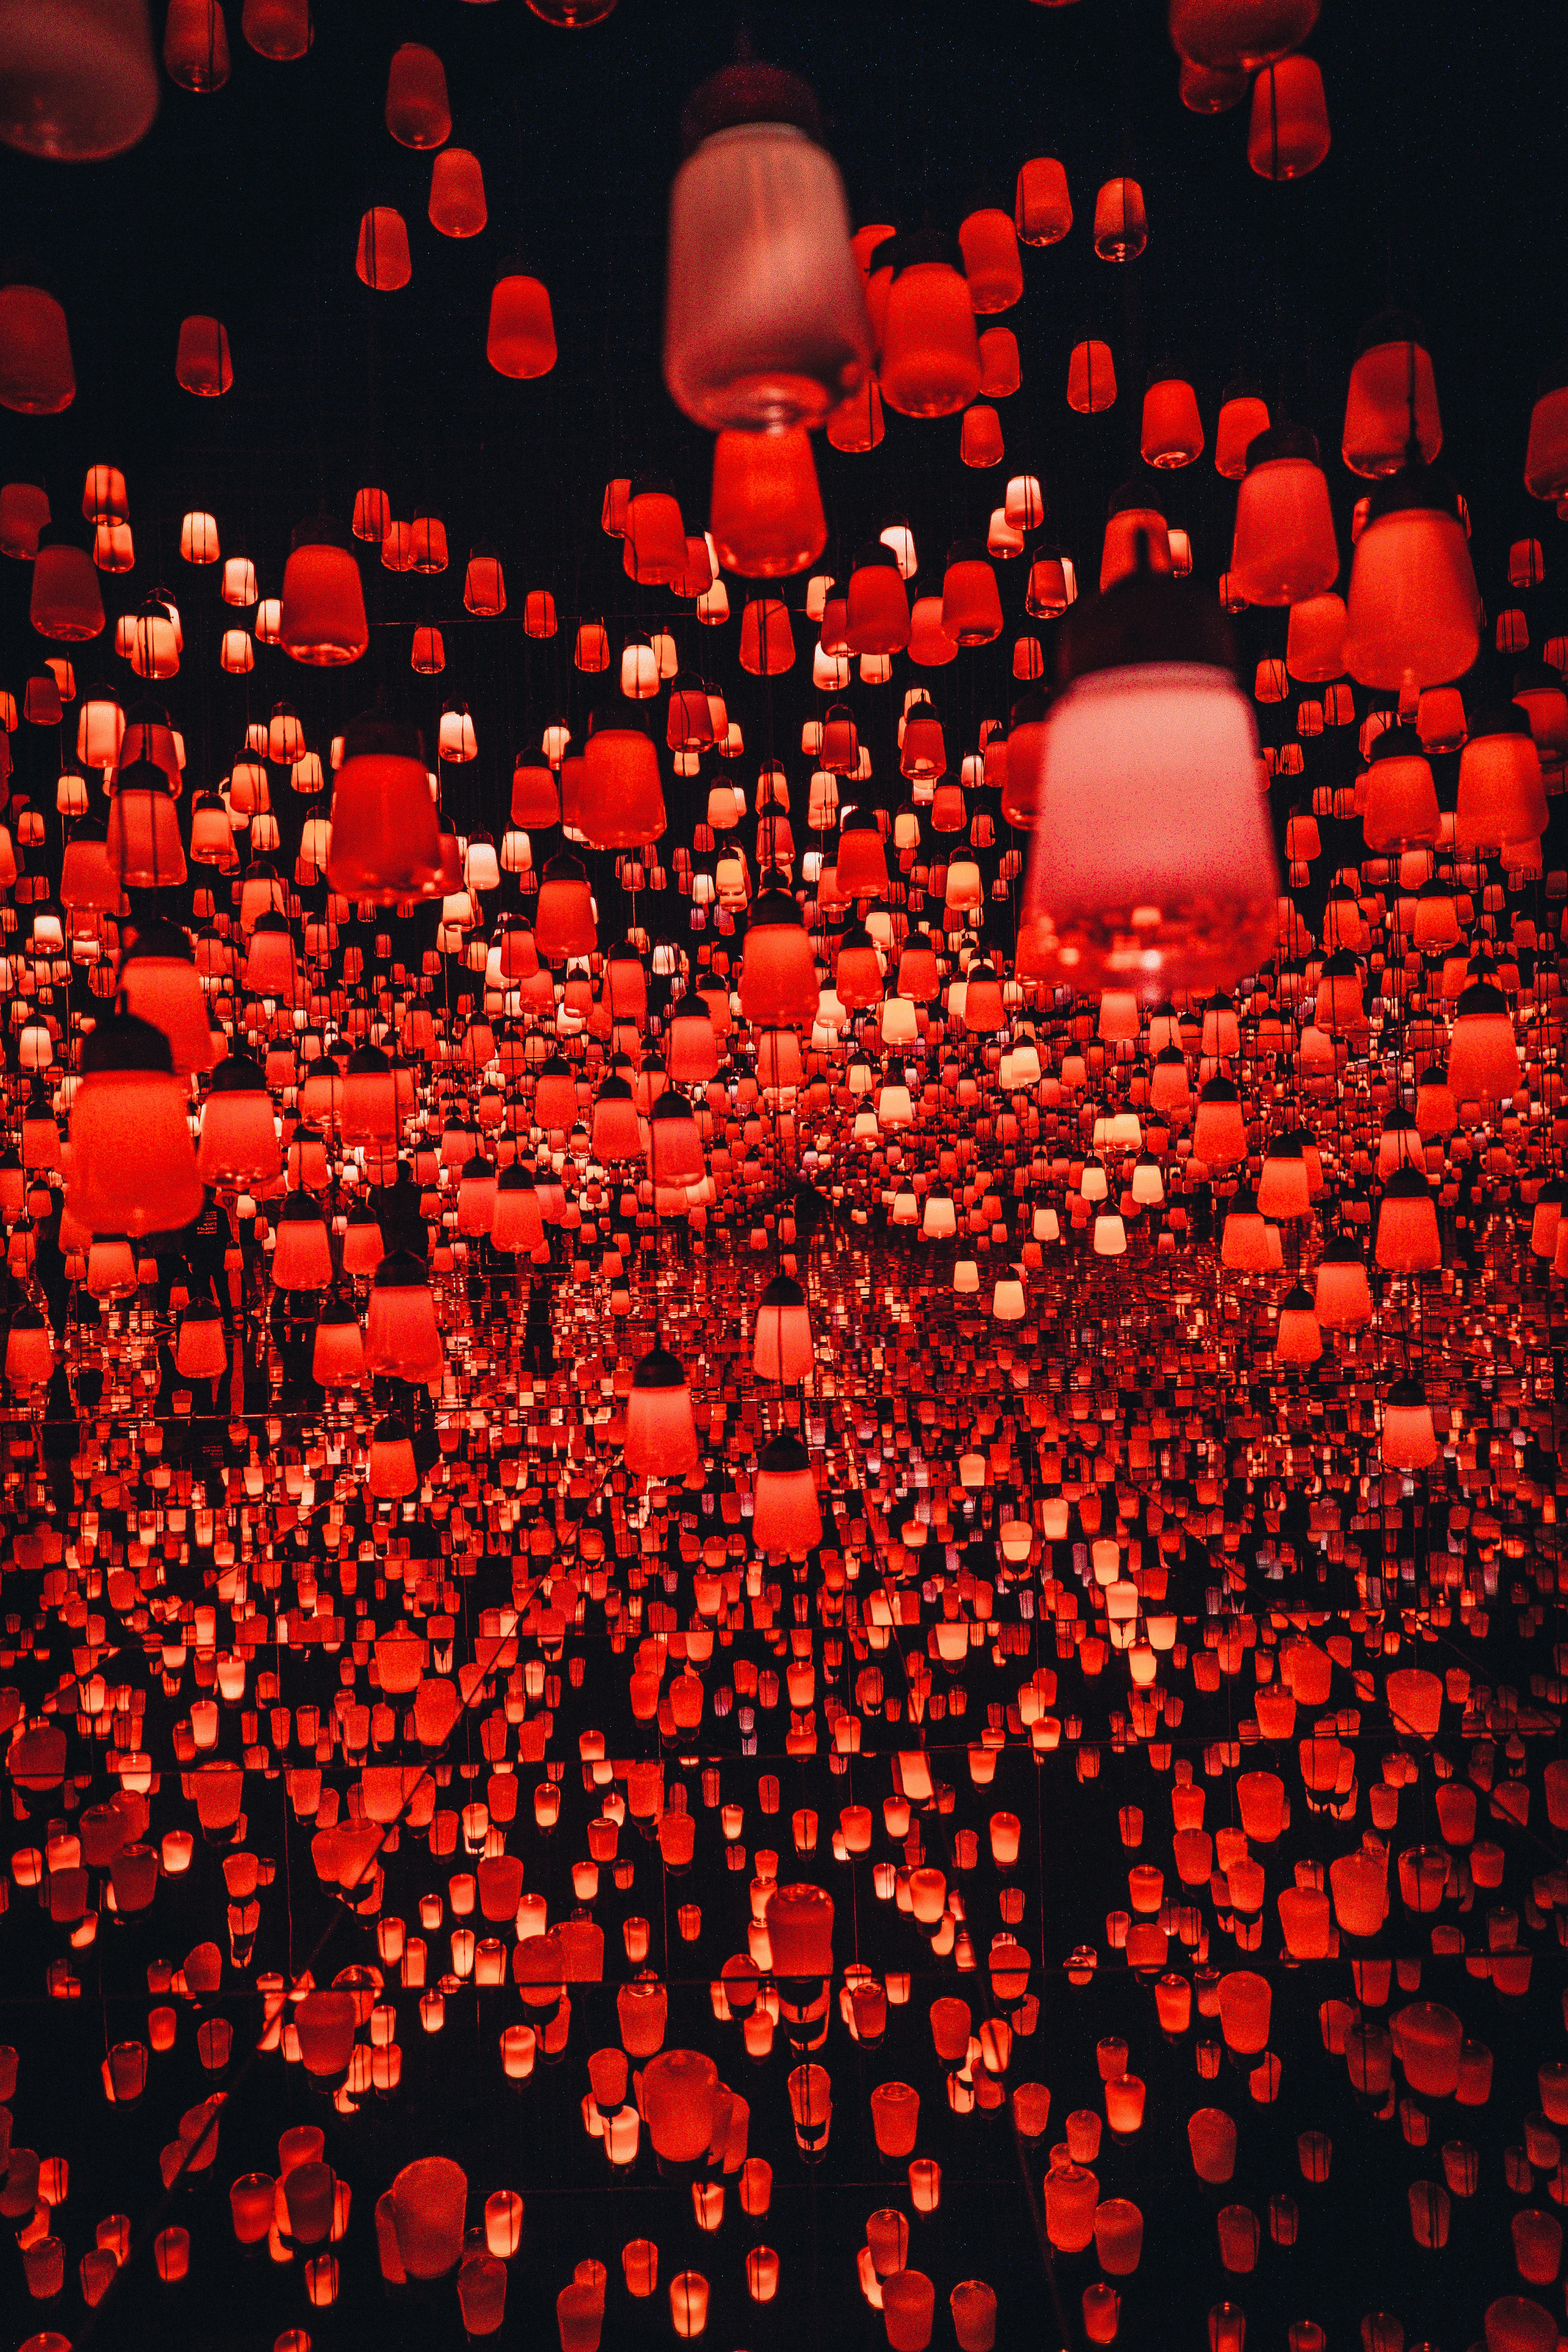
\includegraphics[width=6cm]{Figures/logo}}  %NEW: Changing logo
\def\extraspace{\vspace*{1.6cm}}
\makeatletter
\def\contactdetails{\faicon{phone} & \@telephone \\
                    \faicon{envelope} & \@email}
\makeatother

%%%% FRONT PAGE OF REPORTS

\def\reporttype{Report for}

\long\def\front#1#2#3{
\newpage
\begin{singlespacing}
\thispagestyle{empty}
\vspace*{-1.4cm}
\hspace*{-1.4cm}
\hbox to 16cm{
  \hbox to 6.5cm{\vbox to 14cm{\vbox to 25cm{
    \logo
    \vfill
    \parbox{6.3cm}{\raggedright
      \sf\color[rgb]{0.8, 0.7, 0.1 }    % NEW color 
      {\large\textbf{\name}}\par
      \vspace{.7cm}
      \tabcolsep=0.12cm\sf\small
      \begin{tabular}{@{}ll@{}}\contactdetails
      \end{tabular}
      \vspace*{0.3cm}\par
      ABN: \abn\par
    }
  }\vss}\hss}
  \hspace*{0.2cm}
  \hbox to 1cm{\vbox to 14cm{\rule{4pt}{26.8cm}\vss}\hss\hfill}  %NEW: Thicker line
  \hbox to 10cm{\vbox to 14cm{\vbox to 25cm{   
      \vspace*{3cm}\sf\raggedright
      \parbox{11cm}{\sf\raggedright\baselineskip=1.2cm
         \fontsize{24.88}{30}\color[rgb]{0, 0.29, 0.55}\sf\textbf{#1}}   % NEW: title color blue
      \par
      \vfill
      \large
      \vbox{\parskip=0.8cm #2}\par
      \vspace*{2cm}\par
      \reporttype\\[0.3cm]
      \hbox{#3}%\\[2cm]\
      \vspace*{1cm}
      {\large\sf\textbf{\Date~\Month~\Year}}
   }\vss}
  }}
\end{singlespacing}
\newpage
}

\makeatletter
\def\titlepage{\front{\expandafter{\@title}}{\@author}{\@organization}}
\makeatother

\usepackage{setspace}
\setstretch{1.5}

\usepackage{booktabs}
\usepackage{longtable}
\usepackage{array}
\usepackage{multirow}
\usepackage{wrapfig}
\usepackage{float}
\usepackage{colortbl}
\usepackage{pdflscape}
\usepackage{tabu}
\usepackage{threeparttable}
\usepackage{threeparttablex}
\usepackage[normalem]{ulem}
\usepackage{makecell}
\usepackage{xcolor}


\begin{document}
\titlepage

\{Section 3\}

\hypertarget{research-questions}{%
\section{Research Questions}\label{research-questions}}

\begin{itemize}
\tightlist
\item
  From the data on the number of driver deaths, which time period was the peak, and what historical facts accompany the change after the peak ? How about the trend before and after law introduced ?
\end{itemize}

\hypertarget{data-analysis}{%
\section{Data Analysis}\label{data-analysis}}

\hypertarget{analysis-of-trends-in-driverkilled-before-and-after-1983}{%
\subsection{Analysis of trends in driverkilled before and after 1983}\label{analysis-of-trends-in-driverkilled-before-and-after-1983}}

\includegraphics{report_files/figure-latex/figureE-1.pdf}

According to Figure \ref{fig:figureE}, as we can see, the trend line after 1970 began to decline. The reason is Successive UK governments proposed, but failed to deliver, seat belt legislation throughout the 1970s. Front seat belts were compulsory equipment on all new cars registered in the UK from 1968, although it did not become compulsory for them to be worn until 1983. (\cite{richens2000condoms}) \clearpage

\includegraphics{report_files/figure-latex/Bluebox-1.pdf}

From the figure \ref{fig:Bluebox}, it is clear that the range of monthly deaths among drivers before the law was higher than after it was enacted.

\begin{verbatim}
##       Year          Month    DriversKilled      drivers         front       
##  Min.   :1969   Jan    :15   Min.   : 79.0   Min.   :1309   Min.   : 567.0  
##  1st Qu.:1972   Feb    :14   1st Qu.:108.0   1st Qu.:1511   1st Qu.: 767.0  
##  Median :1976   Mar    :14   Median :121.0   Median :1653   Median : 860.0  
##  Mean   :1976   Apr    :14   Mean   :125.9   Mean   :1718   Mean   : 873.5  
##  3rd Qu.:1979   May    :14   3rd Qu.:140.0   3rd Qu.:1926   3rd Qu.: 986.0  
##  Max.   :1983   Jun    :14   Max.   :198.0   Max.   :2654   Max.   :1299.0  
##                 (Other):84                                                  
##       rear            kms         PetrolPrice        VanKilled           law   
##  Min.   :224.0   Min.   : 7685   Min.   :0.08118   Min.   : 2.000   Min.   :0  
##  1st Qu.:344.0   1st Qu.:12387   1st Qu.:0.09078   1st Qu.: 7.000   1st Qu.:0  
##  Median :401.0   Median :14455   Median :0.10273   Median :10.000   Median :0  
##  Mean   :400.3   Mean   :14463   Mean   :0.10187   Mean   : 9.586   Mean   :0  
##  3rd Qu.:454.0   3rd Qu.:16585   3rd Qu.:0.11132   3rd Qu.:13.000   3rd Qu.:0  
##  Max.   :646.0   Max.   :21040   Max.   :0.13303   Max.   :17.000   Max.   :0  
## 
\end{verbatim}

\begin{verbatim}
##       Year          Month    DriversKilled      drivers         front      
##  Min.   :1983   Feb    : 2   Min.   : 60.0   Min.   :1057   Min.   :426.0  
##  1st Qu.:1983   Mar    : 2   1st Qu.: 85.0   1st Qu.:1171   1st Qu.:516.0  
##  Median :1984   Apr    : 2   Median : 92.0   Median :1282   Median :585.0  
##  Mean   :1984   May    : 2   Mean   :100.3   Mean   :1322   Mean   :571.0  
##  3rd Qu.:1984   Jun    : 2   3rd Qu.:119.0   3rd Qu.:1464   3rd Qu.:629.5  
##  Max.   :1984   Jul    : 2   Max.   :154.0   Max.   :1763   Max.   :721.0  
##                 (Other):11                                                 
##       rear            kms         PetrolPrice       VanKilled          law   
##  Min.   :296.0   Min.   :15511   Min.   :0.1131   Min.   :2.000   Min.   :1  
##  1st Qu.:347.0   1st Qu.:17971   1st Qu.:0.1148   1st Qu.:3.500   1st Qu.:1  
##  Median :408.0   Median :19162   Median :0.1161   Median :5.000   Median :1  
##  Mean   :407.7   Mean   :18890   Mean   :0.1165   Mean   :5.174   Mean   :1  
##  3rd Qu.:471.5   3rd Qu.:19952   3rd Qu.:0.1180   3rd Qu.:7.000   3rd Qu.:1  
##  Max.   :521.0   Max.   :21626   Max.   :0.1201   Max.   :8.000   Max.   :1  
## 
\end{verbatim}

From the tables \ref{tab:Beforelawsub} and \ref{tab:Afterlawsub}
Before law introduced, the median of DriversKilled is 121, the minimum number is 79 and the maximum number is 198. After introduced, the median of DriversKilled is 92, the minimum number is 60 and the maximum number is 154. We can see that the law is effective in helping drivers stay away from death, since it is introduced on 31st January 1983.

\printbibliography

\end{document}
